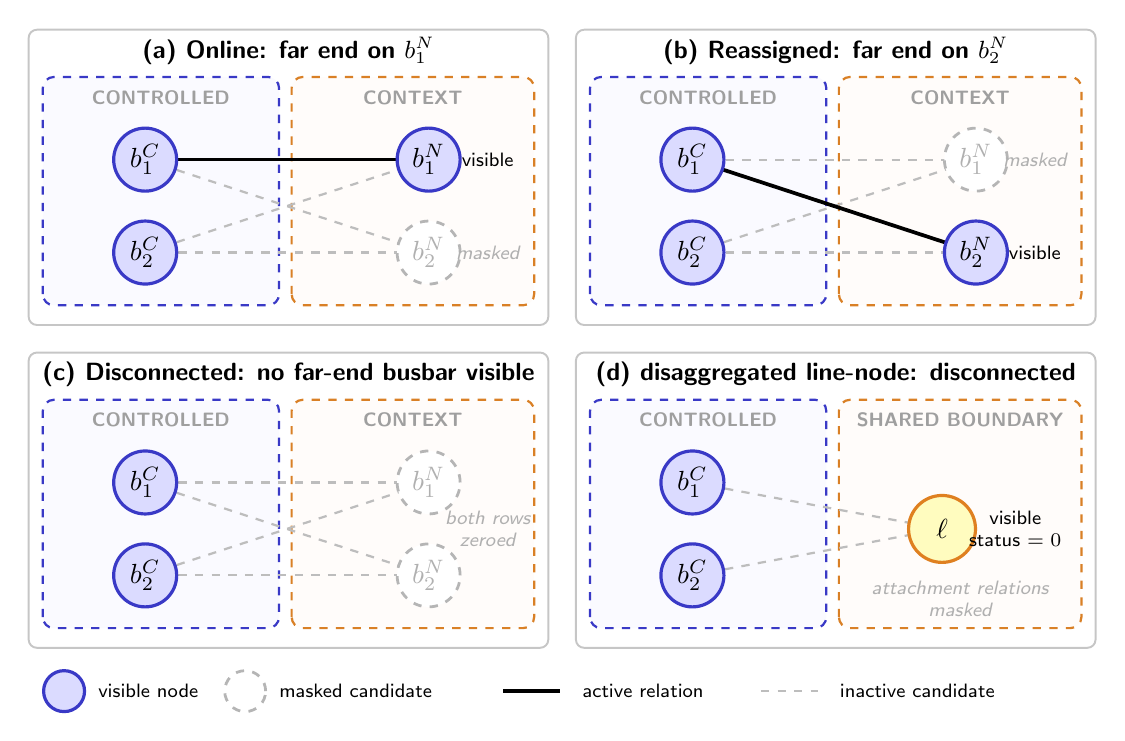
\begin{tikzpicture}[
  x=1cm,
  y=1cm,
  >=stealth,
  font=\sffamily,
  busbar/.style={
    circle,
    draw=blue!55!gray,
    fill=blue!14,
    line width=1.15pt,
    minimum size=8mm,
    inner sep=0pt
  },
  maskedbus/.style={
    circle,
    draw=gray!58,
    fill=white,
    dashed,
    line width=1pt,
    minimum size=8mm,
    inner sep=0pt,
    text=gray!62
  },
  linenode/.style={
    circle,
    draw=orange!75!gray,
    fill=yellow!25,
    line width=1.15pt,
    minimum size=8.5mm,
    inner sep=0pt
  },
  candidate/.style={draw=gray!52, dashed, line width=0.8pt},
  active/.style={draw=black, line width=1.35pt},
  panel/.style={draw=gray!45, rounded corners=3pt, line width=0.7pt},
  controlled/.style={
    draw=blue!55!gray,
    dashed,
    rounded corners=4pt,
    fill=blue!2,
    line width=0.8pt
  },
  context/.style={
    draw=orange!70!gray,
    dashed,
    rounded corners=4pt,
    fill=orange!2,
    line width=0.8pt
  },
  zone/.style={font=\scriptsize\bfseries\sffamily, text=gray!75},
  title/.style={font=\small\bfseries\sffamily},
  note/.style={font=\scriptsize\sffamily, align=center},
  muted/.style={font=\scriptsize\itshape\sffamily, align=center, text=gray!62}
]

% The first three panels share the same four busbar-pair candidates.  Only the
% active relation and the contextual visibility mask change with topology.

% ---------------------------------------------------------------------------
% (a) Boundary line on the first far-end busbar
% ---------------------------------------------------------------------------
\begin{scope}[xshift=0cm,yshift=4.10cm]
  \path[panel] (0,0) rectangle (6.60,3.75);
  \node[title] at (3.30,3.48) {(a) Online: far end on $b^N_1$};
  \path[controlled] (0.18,0.25) rectangle (3.18,3.15);
  \path[context] (3.34,0.25) rectangle (6.42,3.15);
  \node[zone] at (1.68,2.89) {CONTROLLED};
  \node[zone] at (4.88,2.89) {CONTEXT};

  \draw[candidate] (1.48,2.10) -- (5.08,2.10);
  \draw[candidate] (1.48,2.10) -- (5.08,0.92);
  \draw[candidate] (1.48,0.92) -- (5.08,2.10);
  \draw[candidate] (1.48,0.92) -- (5.08,0.92);
  \draw[active] (1.48,2.10) -- (5.08,2.10);

  \node[busbar] at (1.48,2.10) {$b^C_1$};
  \node[busbar] at (1.48,0.92) {$b^C_2$};
  \node[busbar] at (5.08,2.10) {$b^N_1$};
  \node[maskedbus] at (5.08,0.92) {$b^N_2$};
  \node[note] at (5.83,2.10) {visible};
  \node[muted] at (5.83,0.92) {masked};
\end{scope}

% ---------------------------------------------------------------------------
% (b) The far-end busbar assignment changes
% ---------------------------------------------------------------------------
\begin{scope}[xshift=6.95cm,yshift=4.10cm]
  \path[panel] (0,0) rectangle (6.60,3.75);
  \node[title] at (3.30,3.48) {(b) Reassigned: far end on $b^N_2$};
  \path[controlled] (0.18,0.25) rectangle (3.18,3.15);
  \path[context] (3.34,0.25) rectangle (6.42,3.15);
  \node[zone] at (1.68,2.89) {CONTROLLED};
  \node[zone] at (4.88,2.89) {CONTEXT};

  \draw[candidate] (1.48,2.10) -- (5.08,2.10);
  \draw[candidate] (1.48,2.10) -- (5.08,0.92);
  \draw[candidate] (1.48,0.92) -- (5.08,2.10);
  \draw[candidate] (1.48,0.92) -- (5.08,0.92);
  \draw[active] (1.48,2.10) -- (5.08,0.92);

  \node[busbar] at (1.48,2.10) {$b^C_1$};
  \node[busbar] at (1.48,0.92) {$b^C_2$};
  \node[maskedbus] at (5.08,2.10) {$b^N_1$};
  \node[busbar] at (5.08,0.92) {$b^N_2$};
  \node[muted] at (5.83,2.10) {masked};
  \node[note] at (5.83,0.92) {visible};
\end{scope}

% ---------------------------------------------------------------------------
% (c) The physical line is disconnected
% ---------------------------------------------------------------------------
\begin{scope}[xshift=0cm,yshift=0cm]
  \path[panel] (0,0) rectangle (6.60,3.75);
  \node[title] at (3.30,3.48) {(c) Disconnected: no far-end busbar visible};
  \path[controlled] (0.18,0.25) rectangle (3.18,3.15);
  \path[context] (3.34,0.25) rectangle (6.42,3.15);
  \node[zone] at (1.68,2.89) {CONTROLLED};
  \node[zone] at (4.88,2.89) {CONTEXT};

  \draw[candidate] (1.48,2.10) -- (5.08,2.10);
  \draw[candidate] (1.48,2.10) -- (5.08,0.92);
  \draw[candidate] (1.48,0.92) -- (5.08,2.10);
  \draw[candidate] (1.48,0.92) -- (5.08,0.92);

  \node[busbar] at (1.48,2.10) {$b^C_1$};
  \node[busbar] at (1.48,0.92) {$b^C_2$};
  \node[maskedbus] at (5.08,2.10) {$b^N_1$};
  \node[maskedbus] at (5.08,0.92) {$b^N_2$};
  \node[muted] at (5.83,1.51) {both rows\\zeroed};
\end{scope}

% ---------------------------------------------------------------------------
% (d) Explicit-line representation while disconnected
% ---------------------------------------------------------------------------
\begin{scope}[xshift=6.95cm,yshift=0cm]
  \path[panel] (0,0) rectangle (6.60,3.75);
  \node[title] at (3.30,3.48) {(d) disaggregated line-node: disconnected};
  \path[controlled] (0.18,0.25) rectangle (3.18,3.15);
  \path[context] (3.34,0.25) rectangle (6.42,3.15);
  \node[zone] at (1.68,2.89) {CONTROLLED};
  \node[zone] at (4.88,2.89) {SHARED BOUNDARY};

  \draw[candidate] (1.48,2.10) -- (4.65,1.51);
  \draw[candidate] (1.48,0.92) -- (4.65,1.51);
  \node[busbar] at (1.48,2.10) {$b^C_1$};
  \node[busbar] at (1.48,0.92) {$b^C_2$};
  \node[linenode] at (4.65,1.51) {$\ell$};
  \node[note] at (5.58,1.51) {visible\\status $=0$};
  \node[muted] at (4.88,0.62) {attachment relations\\masked};
\end{scope}

% Shared legend.
\node[busbar, minimum size=5.2mm] at (0.45,-0.55) {};
\node[note, anchor=west] at (0.76,-0.55) {visible node};
\node[maskedbus, minimum size=5.2mm] at (2.75,-0.55) {};
\node[note, anchor=west] at (3.06,-0.55) {masked candidate};
\draw[active] (6.03,-0.55) -- (6.75,-0.55);
\node[note, anchor=west] at (6.91,-0.55) {active relation};
\draw[candidate] (9.30,-0.55) -- (10.02,-0.55);
\node[note, anchor=west] at (10.18,-0.55) {inactive candidate};

\end{tikzpicture}
